 % !TEX root = Stanfill_CoDA.tex
\section{Data Application}\label{sec:data}

This data example considers orientations of cubic crystals on a Nickel surface measured by electron backscatter diffraction \citep{bingham10b}. The data were obtained using a 14-fold technical replicate scan of a 10 $\mu$m $\times$ 12.5 $\mu$m Nickel surface at locations spaced 0.2 $\mu$m apart.
The identification of so-called {\it grain maps} -- defined as regions on the surface with nearly identical main direction $\bm S$ -- are often of interest in EBSD data making the estimation of the main direction of rotations, $\bm S$, essential to the field. 
%A central interest in EBSD data is 

In order to demonstrate the impact of different estimators, we calculated all four estimates in each location and found noticeable differences in the results. 
The left hand side of Figure~\ref{fig:grain-map} shows the results for the projected median   $\ProjMedian$: each dot on the surface is colored by  the mis-orientation angle of the  projected median $\ProjMedian$ at this  location.  Distinct spatial structures \blue{resembling grain maps}  are apparent. On the right hand side of the figure shows the angle distance between projected mean and median estimates for each location. Differences are largest along  boundaries between the spatial structures on the left of Figure~\ref{fig:grain-map}. The literature \citep{bingham10b} suggests that distances of $0.5^\circ$ degrees indicate a difference between grains. About 10\% of the locations result in a difference between median and mean estimates of at least that size. 

\begin{figure}[htbp] %  figure placement: here, top, bottom, or page
   \centering
   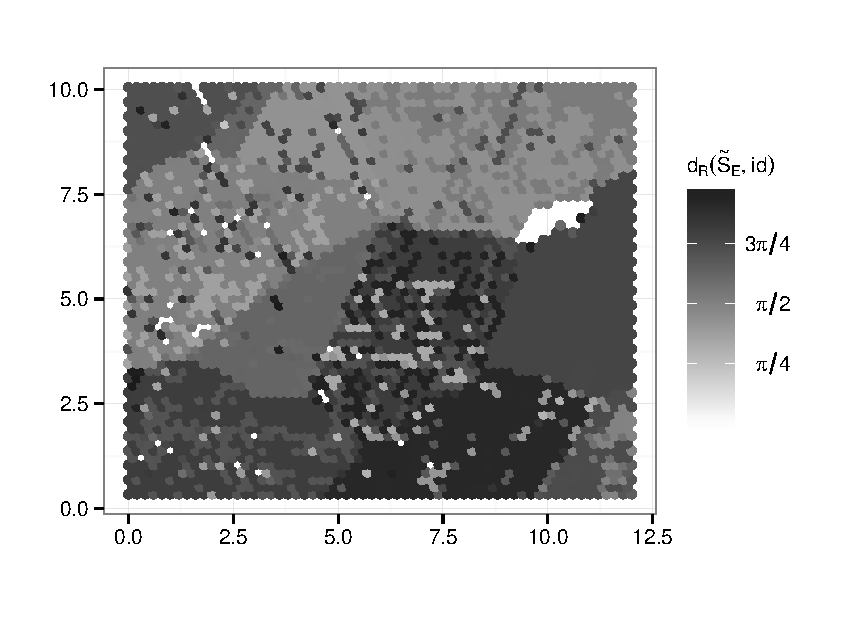
\includegraphics[width=.49\textwidth]{images/grain-map.pdf} 
   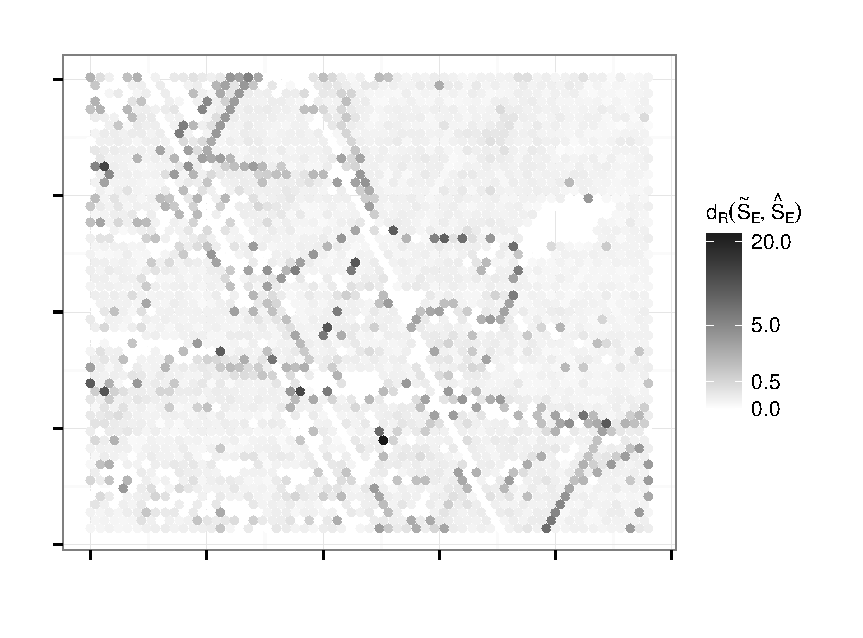
\includegraphics[width=.49\textwidth]{images/grain-diff.pdf} 
   \caption{ \label{fig:grain-map} Overview of all locations of the investigated Nickel surface (left). Each dot corresponds to one location.  Shading shows the angle between $\ProjMedian$ and the identity. On the right, differences between the $\ProjMedian$ and $\ProjMean$ estimates for each location are shown (in degrees). Distances of 0.5$^\circ$ or more are generally considered to be different. Largest differences fall on the boundaries between spatial structures.}
\end{figure}
\vspace{-0.25cm}
\begin{table}[h!]
\caption{\label{tab:rotations} List of all rotations in a single location exhibiting a large difference between mean and median estimators. We observe two clusters of rotations and one outlying rotation. }
\begin{center}
\vspace{-0.5cm}
\scalebox{0.75}{
\begin{tabular}{rrrrrrrrrr}
  \hline
 & $x_{11}$ & $x_{12}$& $x_{13}$& $x_{21}$& $x_{22}$& $x_{23}$& $x_{31}$& $x_{32}$& $x_{33}$ \\ 
  \hline
   & -0.999 & -0.000 & -0.043 & 0.043 & 0.077 & -0.996 & 0.004 & -0.997 & 0.077 \\ 
   & -0.999 & -0.006 & -0.047 & 0.047 & 0.079 & -0.996 & 0.009 & -0.997 & 0.079 \\ 
   & -0.999 & -0.005 & -0.044 & 0.044 & 0.080 & -0.996 & 0.009 & -0.997 & 0.080 \\ 
   & -0.999 & -0.005 & -0.047 & 0.047 & 0.079 & -0.996 & 0.009 & -0.997 & 0.078 \\ 
   & -0.999 & -0.004 & -0.044 & 0.044 & 0.079 & -0.996 & 0.007 & -0.997 & 0.078 \\ 
   & -0.999 & -0.008 & -0.048 & 0.047 & 0.079 & -0.996 & 0.011 & -0.997 & 0.079 \\ 
   & -0.998 & -0.008 & -0.056 & 0.055 & 0.076 & -0.996 & 0.012 & -0.997 & 0.075 \\ 
   & -0.998 & -0.010 & -0.054 & 0.054 & 0.073 & -0.996 & 0.014 & -0.997 & 0.072 \\ [5pt]
   & -0.871 & -0.061 & -0.487 & 0.446 & 0.510 & -0.735 & 0.203 & -0.858 & 0.472 \\ 
   & -0.874 & -0.059 & -0.483 & 0.441 & 0.513 & -0.737 & 0.204 & -0.857 & 0.474 \\ 
   & -0.872 & -0.053 & -0.487 & 0.442 & 0.516 & -0.734 & 0.212 & -0.855 & 0.473 \\ 
   & -0.870 & -0.060 & -0.489 & 0.447 & 0.512 & -0.733 & 0.207 & -0.857 & 0.472 \\ 
   & -0.874 & -0.066 & -0.482 & 0.445 & 0.510 & -0.736 & 0.198 & -0.858 & 0.475 \\ [5pt] 
 & -0.708 & -0.315 & -0.632 & 0.609 & 0.181 & -0.773 & 0.358 & -0.932 & 0.063 \\ 
   \hline
\end{tabular}}
\vspace{-0.5cm}
\end{center}
\end{table}

\noindent In an attempt to explain the difference between the estimates in this example,we focus on the  location with a distance of 15.8$^\circ$, the largest distance between projected mean and median estimate. Figure \ref{fig:pcp} shows a parallel coordinate plot of the rotations at this location: each of the nine coefficients $x_{ij}$ is represented on a separate, vertical axis, Coefficients of the same matrix are connected by a line.  Three clusters of rotation matrices become apparent. Note that the values are jittered -- we use a small perturbation in form of a rotation matrix to draw the rotation matrices in each cluster slightly apart  in order to avoid over-plotting and to demonstrate cluster sizes. The colored lines on top of the rotations show the four estimates of the main direction.  For the numeric form of the data see Table~\ref{tab:rotations}.

\noindent Note that the figure shows a sample of a single location, yet the clustering in the data suggests clearly the presence of \emph{several} main directions. The same holds true for locations in the vicinity which happen to coincide with grain boundaries. 

\noindent This example illustrates that the median estimates, $\ProjMedian$  and $\GeomMedian$, are not nearly as much affected by the clustering in the sample as the means, and reliably estimate the main direction of the largest cluster of rotations within the location.

%\begin{figure}[htbp] %  figure placement: here, top, bottom, or page
%   \centering
%   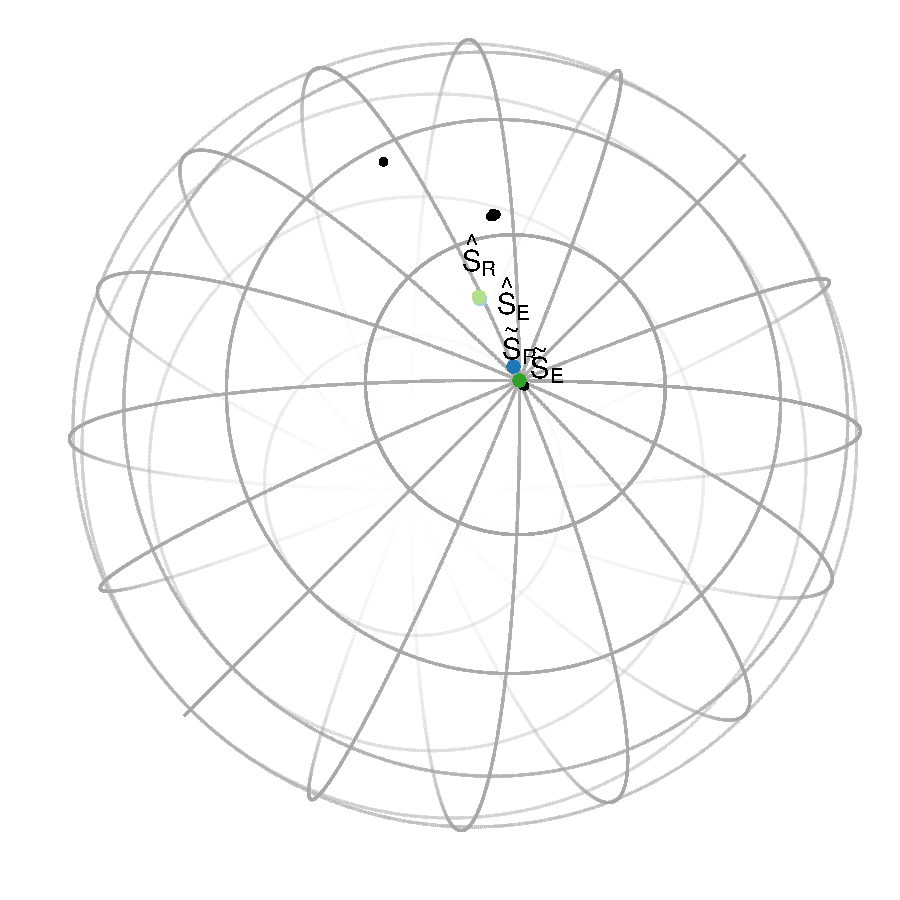
\includegraphics[width=.275\textwidth]{images/eyeball-1031-1.pdf} 
%   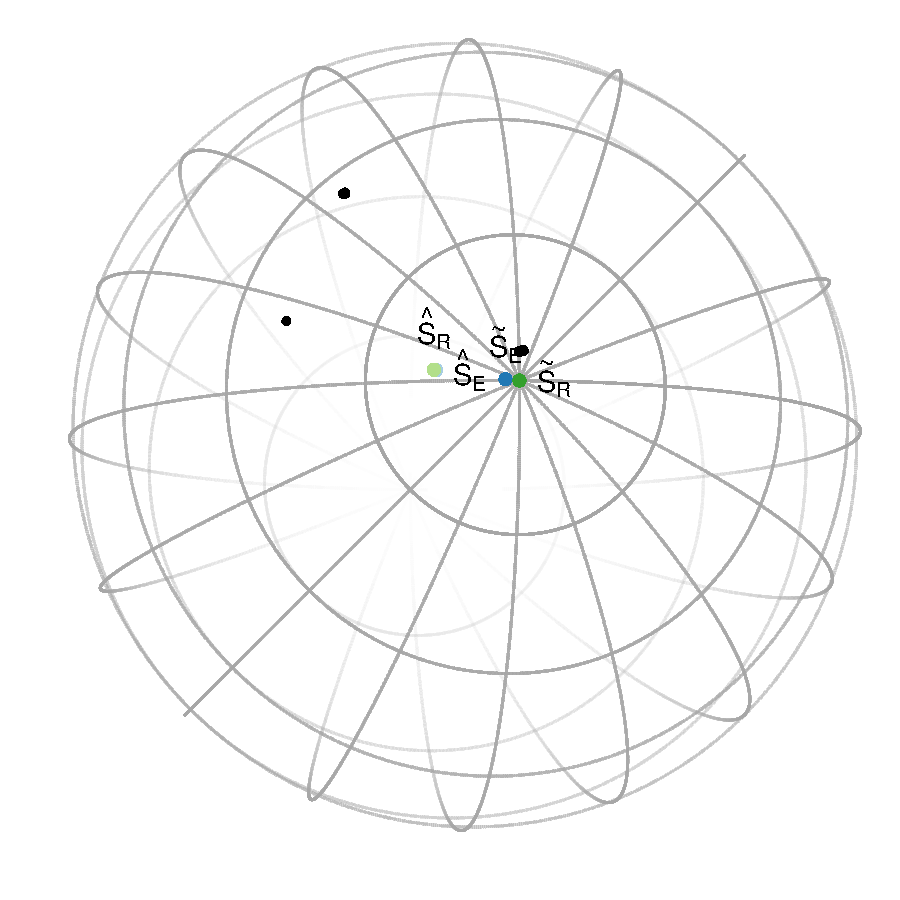
\includegraphics[width=.275\textwidth]{images/eyeball-1031-2.pdf} 
%   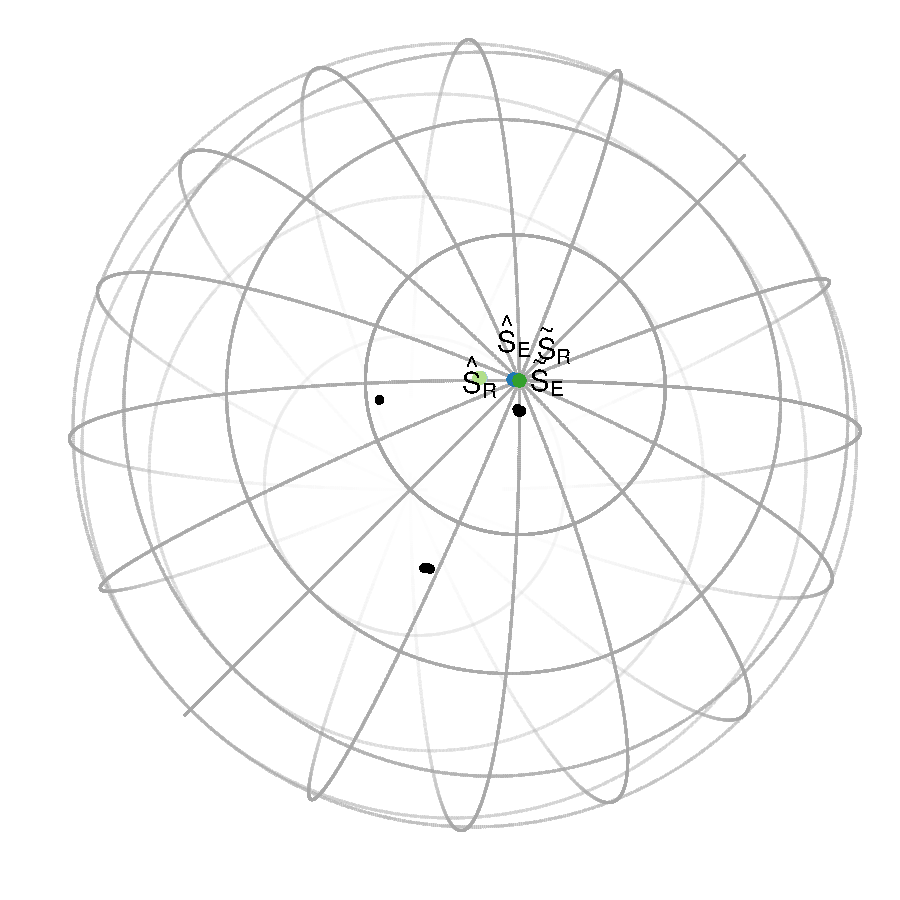
\includegraphics[width=.275\textwidth]{images/eyeball-1031-3.pdf} 
%   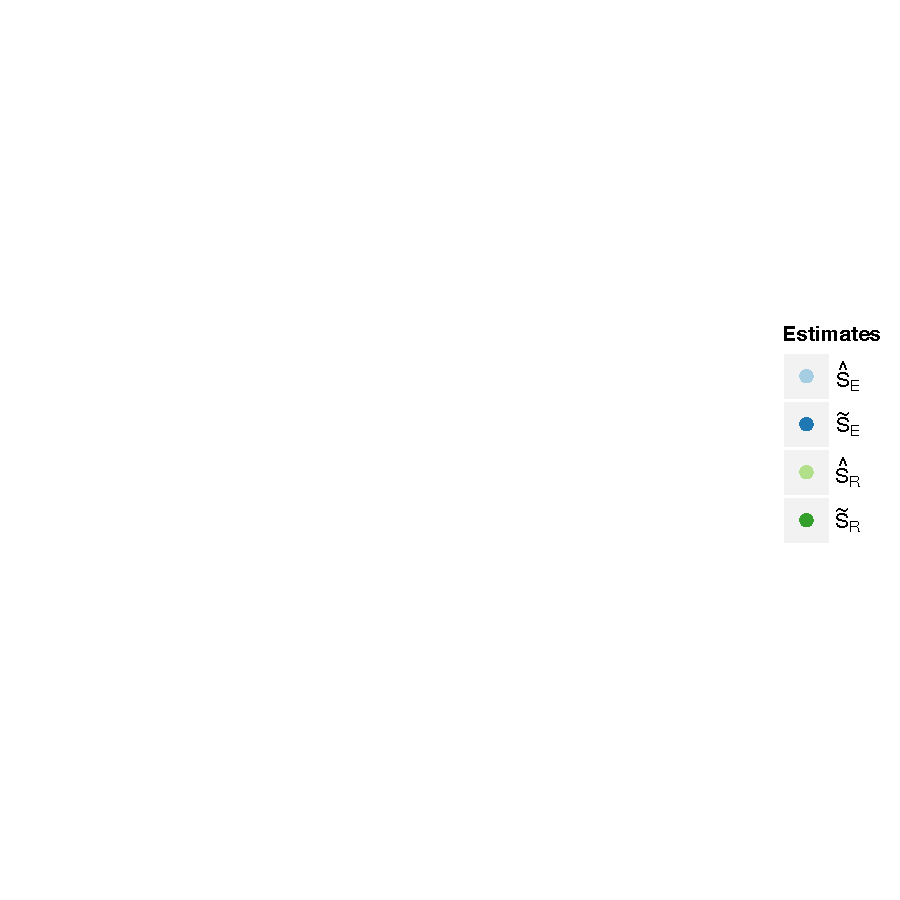
\includegraphics[height=.275\textwidth]{images/legend.pdf} 
%   \caption{ \label{fig:eyeballs-1}Sphere plots of EBSD measurements at a single location. The data sample is shown as dark grey points, the estimates of the main direction are colored and labelled. The clustering of the results makes the existence  of several main directions  quite obvious. }
%\end{figure}

\begin{figure}[htbp] %  figure placement: here, top, bottom, or page
   \centering
   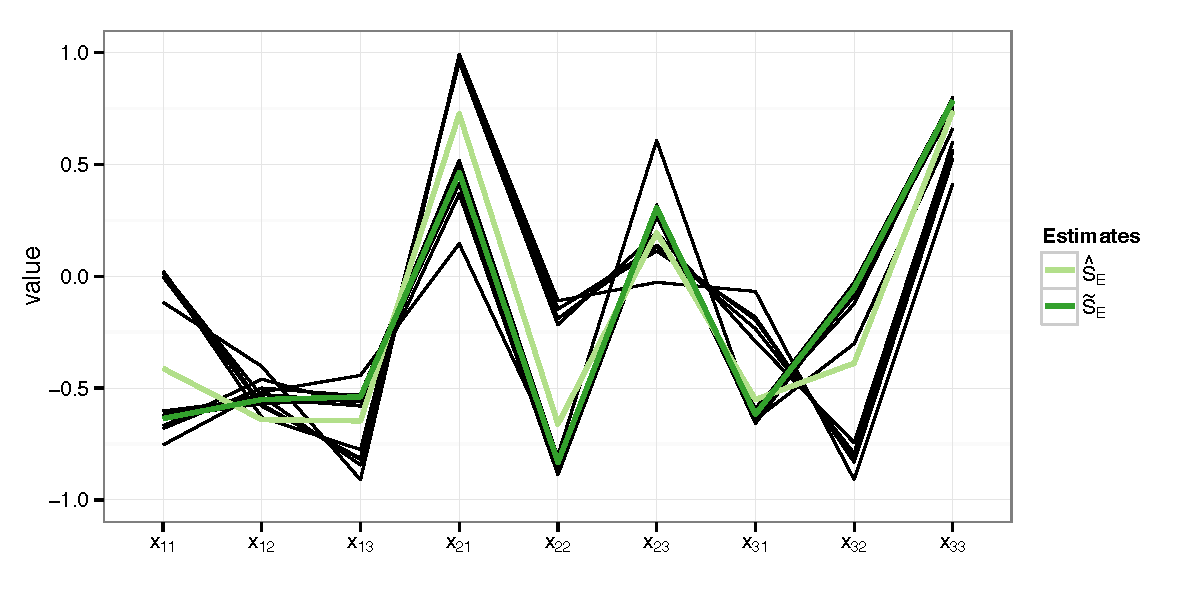
\includegraphics[width=.7\textwidth]{images/pcp.pdf} 
   \caption{ \label{fig:pcp}Parallel coordinate plot of all nine coefficients of the rotation matrices in a single location. Three clusters of rotation matrices are apparent.  }
\end{figure}



